\chapter{Drawing Pack}
\label{app:drawing_pack}

Table~\ref{tab:drawing_tree} presents the hierarchical drawing tree and document breakdown for the Portable Coordinate Measurement Arm (PCMA) electromagnetic joint assembly drawing pack.

\begin{table}[h!]
	\centering
	\small
	\caption{Hierarchical Drawing Tree and Document Index for the PCMA Joint Assembly}
	\label{tab:drawing_tree}
	\vspace{0.2cm}
	\begin{xltabular}{\linewidth}{l p{5.2cm} c p{3.2cm} c}
		\toprule
		\textbf{Drawing Number} & \textbf{Title / Description} & \textbf{Level} & \textbf{Material / Spec.} & \textbf{Qty} \\
		\midrule
	\end{xltabular}
	\vspace{-0.6cm}
	\begin{xltabular}{\linewidth}{l p{5.2cm} c p{3.2cm} c}
		\textbf{24989142-00-00-00} & \textbf{Electromagnetic Brake Joint Assembly} & \textbf{0} & \textbf{Assembly} & \textbf{1} \\
		\midrule
		\quad 24989142-01-00-00 & Joint Shaft & 1 & Aluminium & 1 \\
		\quad 24989142-02-00-00 & Bearing Housing Top & 1 & Aluminium & 2 \\
		\quad 24989142-03-00-00 & Bearing Housing Bottom & 1 & Aluminium & 2 \\
		\quad 24989142-04-00-00 & Joint Housing Bottom Assembly & 1 & Aluminium & 1 \\
		\quad 24989142-05-00-00 & Joint Housing Top-Front & 1 & Aluminium & 1 \\
		\quad 24989142-06-00-00 & Joint Housing Top-Back & 1 & Aluminium & 1 \\
		\quad 24989142-07-00-00 & Base Link Assembly & 1 & Aluminium & 1 \\
		\quad 24989142-08-00-00 & Articulating Link Assembly & 1 & Aluminiumy & 1 \\
		\quad 24989142-09-00-00 & Brake Disc Key & 1 & Brass & 1 \\
		\quad 24989142-10-00-00 & Electromagnet Assembly & 1 & Custom & 1 \\
		\quad 24989142-11-00-00 & Pressure Tab Detail & 1 & Mild Steel & 1 \\
		\quad 24989142-12-00-00 & Friction Plate & 1 & Mild Steel & 1 \\
		\quad 24989142-13-00-00 & Brake Disc & 1 & Wood & 1 \\
		\bottomrule
	\end{xltabular}
\end{table}

\clearpage % Forces the appended drawings to start on a fresh page

% ==============================================================================
% Complete Assembly & Component Drawings
% ==============================================================================
% Settings explained:
% 'pages=-'          : Automatically includes ALL pages from page 1 to the end.
% 'landscape=true'   : Rotates A3 drawings to landscape orientation.
% 'fitpaper=true'    : Resizes the output paper size to match the A3 PDF dimensions.
% 'pagecommand={}'   : Preserves standard page numbering and running headers.
% 'scale=0.92'       : Slightly scales the drawing to fit cleanly within margins.
% ==============================================================================

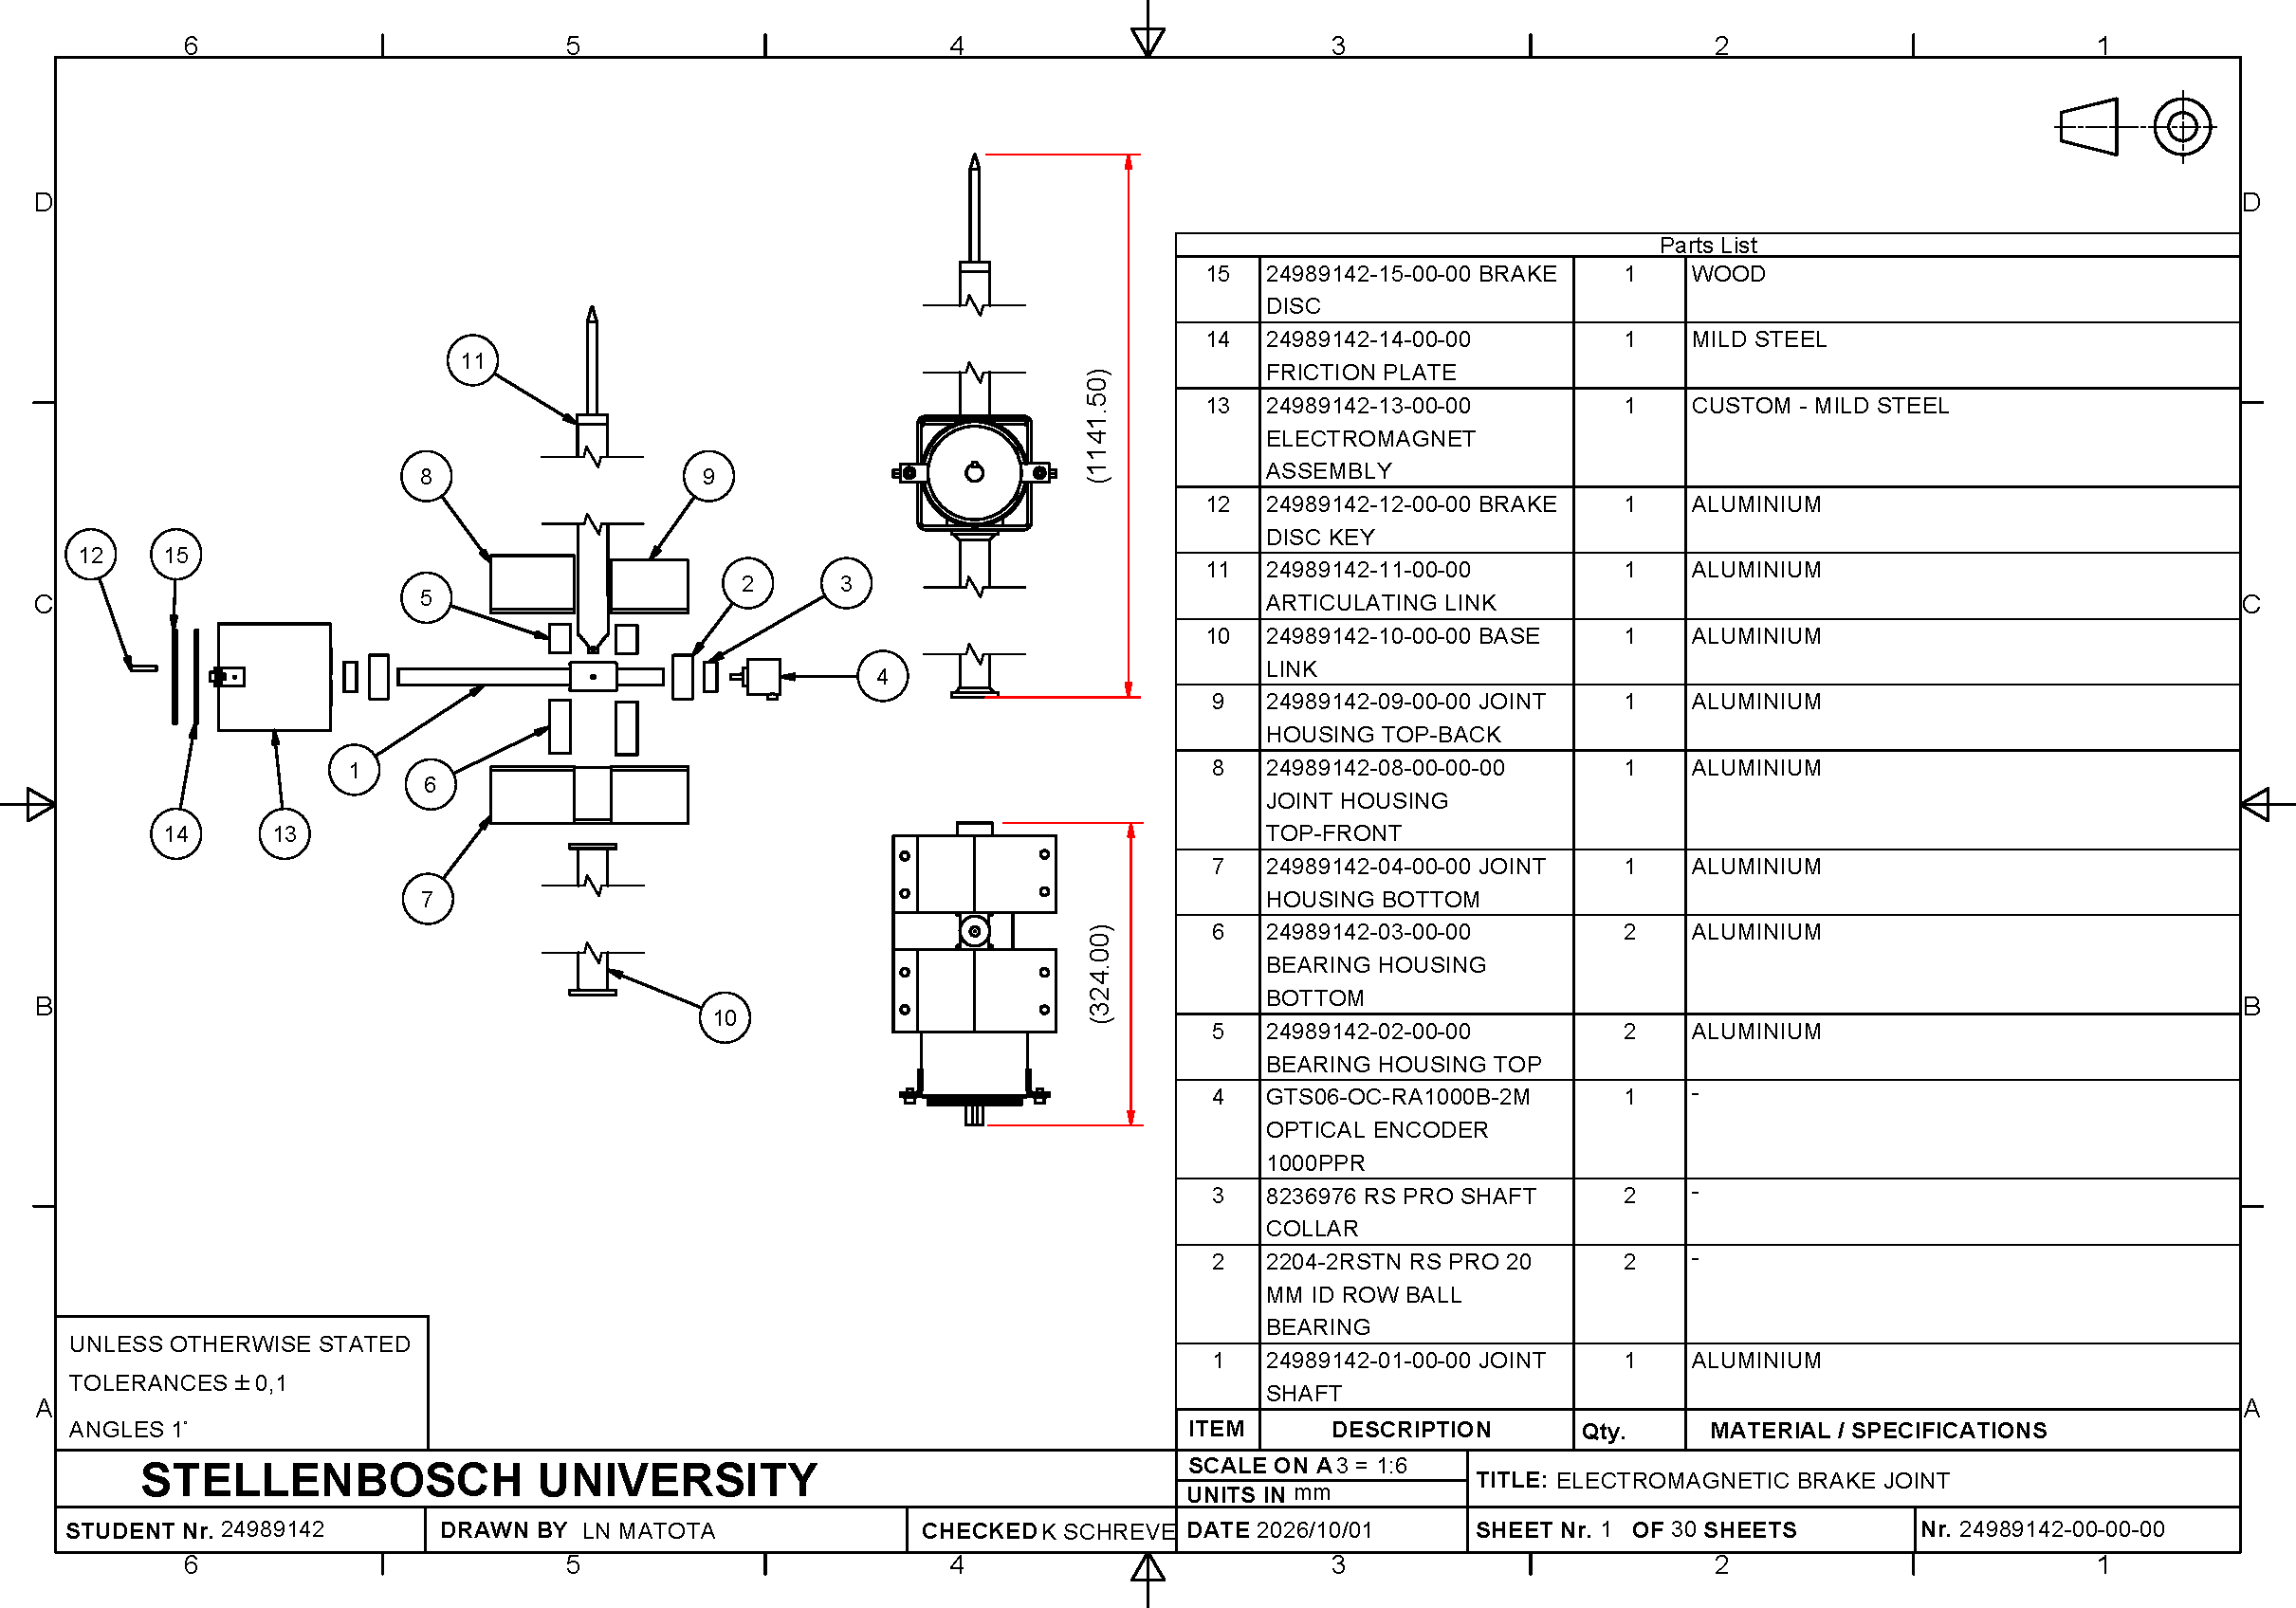
\includepdf[
pages=-,
landscape=true,
fitpaper=true,
pagecommand={\thispagestyle{plain}},
scale=0.92
]{chaps-append/Updated drawing pack.pdf}